%%%%%%%%%%%%%%%%%%%%%%%%%%%%%%%%%%%%%%%%%%%%%%%%%%%%%%%%%%%%%%%%%%%%%%%%%%%%%%%%
%\documentclass[letterpaper, 10 pt, conference]{ieeeconf}
%\documentclass[a4paper, 10pt, conference]{ieeeconf}
%\IEEEoverridecommandlockouts

\documentclass[conference]{IEEEtran}
\IEEEoverridecommandlockouts

%\overrideIEEEmargins

%\pdfobjcompresslevel=0
%\pdfminorversion=4

\usepackage{graphicx}
\usepackage{amsmath}
\usepackage{array}
\usepackage{booktabs}
\usepackage{multirow}
\usepackage{makecell}
\renewcommand\cellalign{lc}
\usepackage{float}
\floatstyle{plain}
\newfloat{equ}{htbp}{loe}
\floatname{equ}{Equation}
\usepackage{tikz}
\usetikzlibrary{arrows.meta, positioning}
\usepackage{tabularx}
\usepackage{caption}
\captionsetup{compatibility=false, labelfont=bf, labelsep=colon} % set style for compatibility with unknown class

%% colocados Omar:
\usepackage{soul}
\usepackage{xcolor}
\usepackage{subcaption}



% --- INICIO DEL BLOQUE DE AHORRO DE ESPACIO ---
% \usepackage{microtype} % Mejora el espaciado entre letras para ahorrar líneas

% % Aprieta el espacio alrededor de las figuras
% \setlength{\textfloatsep}{6pt plus 1.0pt minus 2.0pt}
% \setlength{\floatsep}{6pt plus 1.0pt minus 2.0pt}
% \setlength{\intextsep}{6pt plus 1.0pt minus 2.0pt}
% \setlength{\abovecaptionskip}{4pt plus 1pt minus 1pt} % Espacio antes del caption
% \setlength{\belowcaptionskip}{-5pt} % Espacio después del caption (negativo para subir el texto)


% Aprieta ligeramente los títulos de sección
% \usepackage[compact]{titlesec}
% \titlespacing{\section}{0pt}{6pt plus 2pt minus 2pt}{4pt plus 2pt minus 2pt}
% \titlespacing{\subsection}{0pt}{5pt plus 2pt minus 2pt}{3pt plus 2pt minus 2pt}

%%%%%%%%%%%%%%%%%%%%%%%%%%%%%%%%%%%%%%%%%%%%%%%%%%%%%%%%%%%%%%%%%%%%%%%%%%%%%%%%

\title{\LARGE \bf
Validation of a Theta/Alpha (Fz/Pz) EEG-Based Cognitive Load Index for Workload-Aware Human--Machine Systems
}

\author{%
\parbox{\linewidth}{\centering
Edgar R. Hernandez-Rios$^{1,2}$, J. Aparicio-Juarez$^{1}$, Omar A. Dominguez-Ramirez$^{1}$, and Christian Penaloza$^{2,3}$\\
\vspace{1mm}
$^{1}$Universidad Autonoma del Estado de Hidalgo (UAEH), Mexico\\
$^{2}$Mirai Innovation Research Institute, Osaka, Japan\\
$^{3}$Universidad Autonoma de Chihuahua (UACH), Mexico
}
%
}

\newcolumntype{C}{>{\centering\arraybackslash}X}
% Configuración del estilo del título para que sea más estético y compacto
\captionsetup[table]{
  labelfont={bf,small},
  textfont={it,small},
  justification=justified,
  singlelinecheck=false,
  labelsep=period,
  skip=5pt
}
\begin{document}
\maketitle
\thispagestyle{empty}
\pagestyle{empty}

%%%%%%%%%%%%%%%%%%%%%%%%%%%%%%%%%%%%%%%%%%%%%%%%%%%%%%%%%%%%%%%%%%%%%%%%%%%%%%%%
\begin{abstract}
Workload-aware intelligent human--machine systems require reliable and interpretable user-state estimation mechanisms. This study validates an EEG-based cognitive load index defined as the ratio of frontal theta to parietal alpha power ($\theta_{Fz}/\alpha_{Pz}$) across two complementary paradigms: a controlled laboratory benchmark and an ecological interactive task.

In the controlled paradigm, passive reading (low demand) and Stroop interference (high demand) were used to manipulate workload. Six sessions satisfying predefined signal-quality criteria consistently exhibited higher $\theta_{Fz}/\alpha_{Pz}$ ratios during high demand, with group means increasing from 1.37 (SD = 1.80) to 4.65 (SD = 4.99) and a paired Cohen's $d=0.75$, supporting discriminative validity under well-defined conditions. In the ecological paradigm, the index was baseline-normalized during interactive task execution; 6 of 8 sessions showed increased ratios relative to baseline, indicating sensitivity to task engagement under realistic interaction variability.

NASA-TLX scores were collected to contextualize perceived workload, and an exploratory comparison with the EEG-based index in the participants with both measures showed positive but non-significant correlations consistent with the expected direction. Within the constrained conditions examined here, the results support the $\theta_{Fz}/\alpha_{Pz}$ ratio as a compact and interpretable metric that exhibits a consistent directional sensitivity to differences in cognitive workload, with broader generalization requiring further data accumulation and more rigorous validation before its deployment in workload-aware human--machine systems.
\end{abstract}

%Cambio sugerido
% \begin{keywords}
% Electroencephalography (EEG), Cognitive load, Brain-computer interfaces, theta/Alpha ratio, Stroop task, Exergaming, Human–machine interaction, Lab Streaming Layer (LSL).
% \end{keywords}
%Cambio sugerido
\begin{keywords}
Electroencephalography (EEG), Cognitive load estimation, Theta/Alpha ratio, User-state estimation, Workload-aware systems, Human--machine interaction, Neuroergonomics, Exergaming.
\end{keywords}


% Otras kewwords válidas

%Cognitive load
%Electroencephalography (EEG)
%theta/Alpha ratio
%Fronto-parietal dynamics
%Workload assessment
%Human–machine interaction
%Neuroergonomics
%Experimental validation
%Adaptive systems
%Brain monitoring
%Spectral power analysis
%Neural oscillations
%Cortical dynamics
%Mental effort
%Biomarkers
%Index validation
%Signal processing
%Physiological measurement
%Real-time monitoring
%Intelligent interfaces
%User-state estimation
%Exergaming / Interactive paradigms

% Keywords Rafa
%\begin{keywords}
%EEG, Cognitive load, theta/alpha ratio, Stroop task, exergaming, haptic interface, Lab Streaming Layer (LSL).
%\end{keywords}

%%%%%%%%%%%%%%%%%%%%%%%%%%%%%%%%%%%%%%%%%%%%%%%%%%%%%%%%%%%%%%%%%%%%%%%%%%%%%%%%
\section{Introduction}

Quantifying cognitive load from neurophysiological signals is a central challenge in neuroergonomics, adaptive human--machine interaction, and intelligent training systems. Reliable workload estimation provides a foundation for understanding how task demands influence attention, executive control, and performance, and is a prerequisite for the development of systems that respond appropriately to user state \cite{24}. Among available sensing modalities, electroencephalography (EEG) is particularly attractive due to its high temporal resolution and its direct relationship with cortical processes underlying mental effort and cognitive control.

A substantial body of literature has established robust associations between spectral EEG features and cognitive workload. In particular, increases in frontal theta activity (4--7~Hz) have been linked to sustained attention, conflict monitoring, and executive control~\cite{c8}, while decreases in parietal alpha activity (8--12~Hz) are commonly interpreted as markers of increased task engagement and information processing demand. Recent meta-analyses and systematic reviews have confirmed that these spectral modulations constitute some of the most consistent EEG correlates of cognitive load across tasks and populations~\cite{c1,c4}.

Building on these findings, ratio-based EEG indices combining theta and alpha power have been proposed as compact and interpretable measures of mental workload. Theta-to-alpha and alpha-to-theta ratios integrate complementary neural mechanisms into a single scalar metric, offering practical advantages for monitoring workload trends with reduced feature dimensionality~\cite{c1,c7}. However, recent studies have emphasized that the reliability and stability of such indices depend strongly on methodological choices, including electrode selection, preprocessing pipelines, artifact handling, and task context~\cite{c4,c6}. Consequently, clearly defined and reproducible validation protocols remain essential, particularly when extending EEG-based workload indices beyond tightly controlled laboratory settings.

Controlled interference paradigms, such as the Stroop task, continue to serve as standard benchmarks for eliciting well-characterized increases in cognitive load. EEG studies consistently report frontal theta increases and parietal alpha decreases during Stroop interference, reflecting elevated executive and attentional demands~\cite{c5,c9}. While such paradigms are well suited for validating workload indices under controlled conditions, there is increasing interest in examining whether these indices retain sensitivity in more ecological and interactive scenarios, where task structure is less rigid and user engagement may vary dynamically~\cite{c2,c3}.

In this work, we evaluate an EEG-based cognitive load index defined as the ratio of frontal theta power at Fz to parietal alpha power at Pz. The index is examined across two complementary paradigms: (i) a controlled laboratory protocol contrasting low cognitive load (passive reading) and high cognitive load (Stroop interference), and (ii) an ecological interactive exergaming task implemented on a human--robotic physical interaction platform. A common acquisition and processing pipeline with explicit signal-quality criteria is applied across paradigms. The controlled paradigm is used to establish discriminative validity under well-defined conditions, while the ecological paradigm is used to explore the sensitivity of the same index to task engagement in a naturalistic interactive context.

While the Theta/Alpha ratio itself is an established spectral measure, the contribution of this work is not the index per se but its \emph{systematic, end-to-end validation} under a single, fully reported acquisition and preprocessing pipeline (low-cost 8-channel device, LSL streaming, fixed notch/bandpass filtering, Welch PSD with 1~s windows, multi-criterion artifact handling, and explicit signal-quality inclusion criteria) applied identically to a controlled benchmark and to an ecological human--robotic interactive task. The main contributions are: (i) controlled validation of the Theta/Alpha (Fz/Pz) ratio with explicit signal-quality criteria and effect size estimation; (ii) baseline-normalized evaluation in an ecological exergaming task; (iii) a transparent, reproducible pipeline for spectral estimation and artifact handling across contexts that addresses the methodological dependencies emphasized in recent reviews~\cite{c4,c6}; and (iv) an explicit, descriptive comparison between the EEG-derived index and subjective workload (NASA-TLX) in the subset of participants with both measures, used to contextualize but not to overstate the convergence between objective and self-reported workload. Within these constrained conditions, the index is shown to exhibit a consistent directional sensitivity to differences in cognitive workload across both paradigms.


%%%%%%%%%%%%%%%%%%%%%%%%%%%%%%%%%%%%%%%%%%%%%%%%%%%%%%%%%%%%%%%%%%%%%%%%%%%%%%%%
\section{Interactive Exergaming Platform and Task Context}

To examine the behavior of the proposed EEG-based cognitive load index under ecological conditions, an interactive exergaming platform was employed as the task context. Exergaming environments provide structured yet flexible contexts in which cognitive demand emerges from sustained attention, sensorimotor coordination, and continuous interaction, rather than from strictly scripted stimuli~\cite{14,15}. The platform used in this study, referred to as \emph{K9 Canine Quest}, was developed at the Advanced Robotics and Haptic Interfaces Laboratory (UAEH) as a modular interactive system integrating virtual environments, multiple input modalities, and force-feedback interaction~\cite{16}. In the present work it is used solely as an experimental task environment (not as a therapeutic or clinical intervention), and the inclusion of haptic interaction is motivated by prior work on force-feedback coupling between user motion and virtual task dynamics~\cite{22,23}. Users navigate and interact with on-screen elements while maintaining attention and responding to dynamic feedback, so that cognitive demand arises from the coordination of perception, decision-making, and motor actions, with natural variability in strategies, pacing, and engagement.


\begin{figure}[t]
\centering
\begin{subfigure}[t]{0.48\columnwidth}
\centering

\includegraphics[width=\linewidth]{figures/CQuest1.jpg}
\caption{Virtual environment used during the exergaming task.}
\end{subfigure}
\hfill
\begin{subfigure}[t]{0.48\columnwidth}
\centering
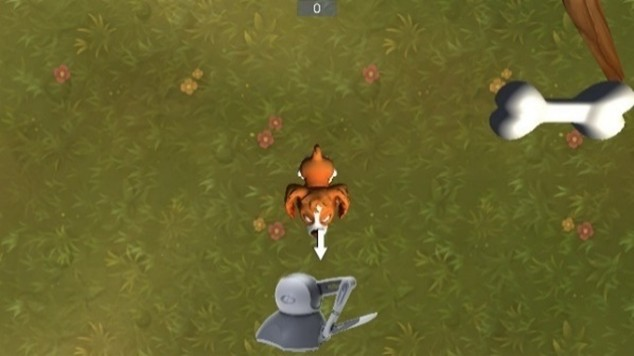
\includegraphics[width=\linewidth]{figures/CQuest2.jpg}
\caption{Haptic interface providing force-feedback interaction.}
\end{subfigure}
\vspace{0.4em}
\begin{subfigure}[t]{0.6\columnwidth}
\centering
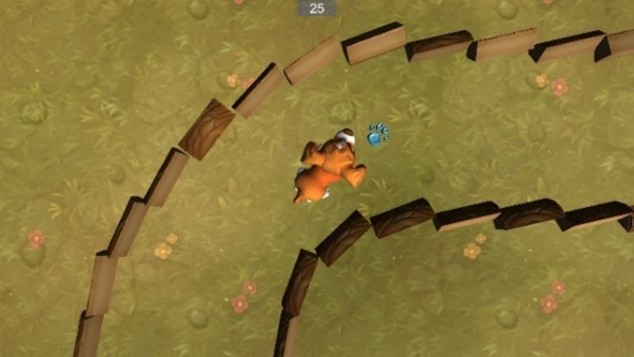
\includegraphics[width=\linewidth]{figures/CQuest4.jpg}
\caption{Participant interacting with the system during gameplay.}
\end{subfigure}
\caption{K9 Canine Quest exergaming platform used as an ecological interactive task environment. The system integrates virtual stimuli, haptic interaction, and user movement to create a physically and cognitively engaging task context while EEG signals are recorded.}
\label{fig:exergaming_platform}
\end{figure}

The platform supports keyboard, gamepad, and haptic interaction modalities; in this study, interaction modality is treated as part of the ecological variability of the task rather than as an independent experimental factor, and analyses are conducted at the session level. The exergaming task is not evaluated in terms of efficacy, training outcomes, or clinical impact; rather, it is used as a representative interactive scenario that introduces realistic sources of variability (movement-related artifacts, fluctuating attention, individual interaction strategies) under which the EEG-based Theta/Alpha (Fz/Pz) index can be assessed.



%%%%%%%%%%%%%%%%%%%%%%%%%%%%%%%%%%%%%%%%%%%%%%%%%%%%%%%%%%%%%%%%%%%%%%%%%%%%%%%%
\section{Methods}

\subsection{Participants and data overview}
EEG was collected in a controlled protocol (14 sessions; 6 includable) and an ecological exergaming task (8 sessions). Analyses were session-level (some participants contributed multiple sessions). All participants provided informed consent under institutional procedures.

\subsection{EEG acquisition hardware and software}
EEG was recorded using the AURA device, an 8-channel EEG system with a nominal sampling rate of 250~Hz. Signals were streamed in real time using Lab Streaming Layer (LSL). A custom graphical interface implemented in PyQt5 was used to guide the experimental protocols and store recorded data as CSV files. Electrodes were positioned according to the international 10--20 system at Fp1, Fp2, F3, Fz, F4, P3, Pz, and P4, covering bilateral frontopolar, frontal, and parietal regions as well as the midline. The cognitive load index was computed using theta-band activity from Fz and alpha-band activity from Pz, selected based on prior evidence linking frontal theta and parietal alpha dynamics to cognitive workload.

\subsection{Offline preprocessing}
All EEG data were processed offline using a standardized preprocessing pipeline. Signals were notch filtered at 60~Hz (Q~=~30) to attenuate power line interference, followed by bandpass filtering between 1 and 40~Hz using a fourth-order Butterworth filter.

Common average reference (CAR) was applied in the ecological paradigm to improve robustness under movement-related noise inherent to interactive tasks. For the controlled paradigm, data were analyzed using the original reference configuration to preserve comparability with the acquisition setup and minimize additional signal transformations.

The effective sampling rate was assumed to be 250~Hz and was verified when necessary using signal timestamps.

\subsection{Spectral analysis and Cognitive Load Index (CLI)}
Spectral power was estimated using Welch’s power spectral density (PSD) method. EEG signals were segmented into windows of 250 samples (1~s at 250~Hz) with 50\% overlap (step size of 125 samples). For each window, theta-band power (4--7~Hz) was computed from channel Fz, and alpha-band power (8--12~Hz) from channel Pz. Bandpower was defined as the integral of the PSD over the corresponding frequency band using the trapezoidal rule.

The cognitive load index was defined for each window as:

\begin{equation}
\mathrm{Index} = \frac{\theta_{Fz}}{\alpha_{Pz}}.
\label{CLI2}
\end{equation}

Non-finite values were discarded and division by zero was avoided. Index values were averaged across valid windows within each phase or session.

An overview of the EEG processing pipeline and index computation is shown in Fig.~\ref{fig:pipeline}.
\begin{figure}[H] % El asterisco hace que abarque dos columnas. [t!] fuerza la posición arriba.
    \centering
    % Ajusta el width si es necesario (0.85\linewidth suele verse bien)
    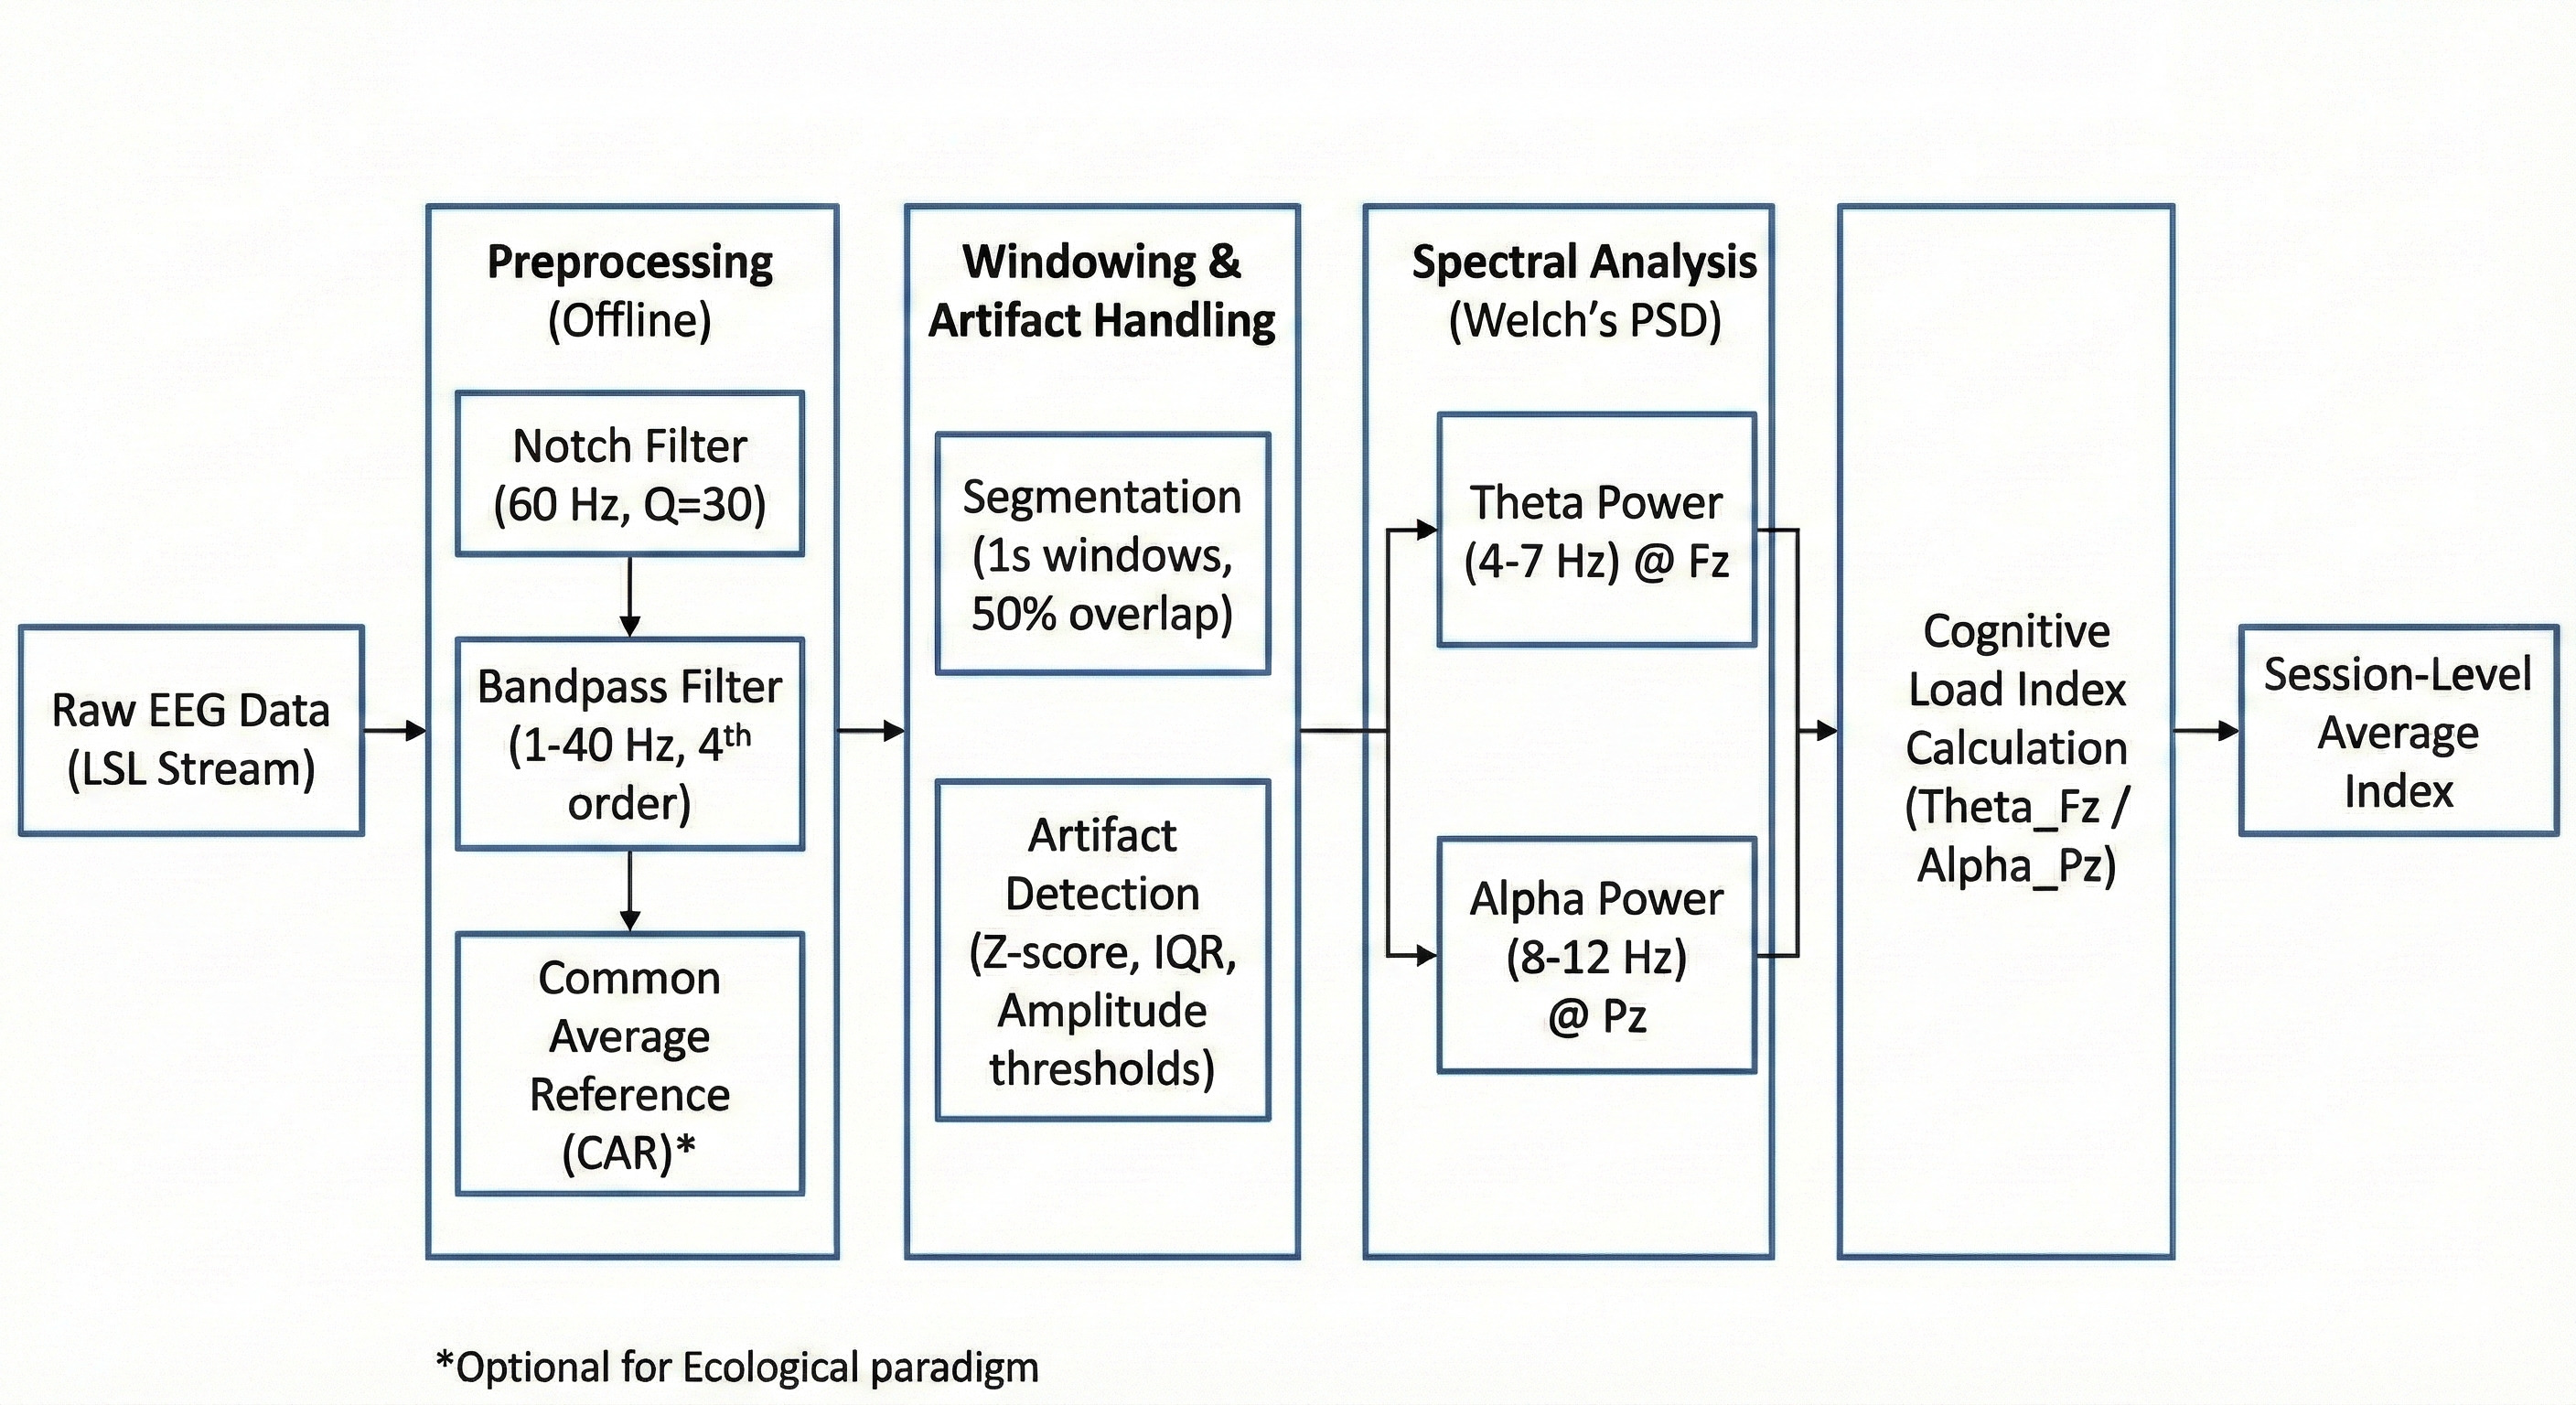
\includegraphics[width=0.9\linewidth]{figures/pipeline1.jpg} 
    \caption{Overview of the EEG processing pipeline and cognitive load index computation. The pipeline includes preprocessing, artifact handling, spectral feature extraction (theta at Fz, alpha at Pz), and index calculation. The asterisk (*) notes steps specific to the ecological paradigm.}
    \label{fig:pipeline}
\end{figure}

\subsection{Artifact detection and window selection}
Artifacts were detected independently for channels Fz and Pz using three criteria: Z-score threshold (3), interquartile range (IQR) threshold (multiplier of 3), and absolute amplitude threshold (200~$\mu$V). Artifact-contaminated samples were handled using linear interpolation to preserve temporal continuity when sufficient surrounding data were available; segments with excessive contamination were excluded from analysis.

After artifact handling, the cognitive load index was recomputed. Only windows with finite index values within a predefined range (0.01--100) were retained. A minimum of two valid windows per phase was required to compute session-level averages, ensuring that estimates reflected more than isolated spectral events.

In some sessions, strict artifact rejection resulted in a limited number of valid analysis windows. This reflects the conservative nature of the predefined signal-quality criteria, particularly under conditions of frontal or parietal contamination. Because the objective of this study was to evaluate session-level trends and discriminative directionality of the index rather than window-level inference, sessions with a minimum of two valid windows were retained to avoid discarding usable recordings while preserving methodological transparency.


\subsection{Controlled paradigm: low vs.\ high cognitive load}
The controlled paradigm followed a baseline--low--high protocol. After a signal verification phase, participants completed a baseline consisting of 90~s with eyes open followed by 90~s with eyes closed. The low cognitive load condition consisted of passive reading for approximately 3~minutes. The high cognitive load condition consisted of a Stroop color--word interference task of similar duration, in which participants identified the ink color rather than the written word using keyboard inputs (R/B/G/Y).

A session was considered \emph{includable} if, in both low and high load phases, the artifact percentage in either Fz or Pz did not exceed 50\% and at least two valid analysis windows remained after cleaning. Among includable sessions, the hypothesis tested was that the mean cognitive load index would be higher in the high-demand condition than in the low-demand condition (High $>$ Low).

\subsection{Subjective cognitive load assessment: NASA-TLX}
Subjective cognitive workload was assessed using the NASA Task Load Index (NASA-TLX), a multidimensional questionnaire capturing Mental Demand, Physical Demand, Temporal Demand, Performance, Effort, and Frustration. Raw (unweighted) NASA-TLX scores were computed and reported as percentages (0--100).

For the controlled paradigm, NASA-TLX was collected as a single global score per participant reflecting the overall session. Consequently, NASA-TLX was not used for within-session Low vs.\ High comparisons. However, for the subset of participants with both a global NASA-TLX score and a valid EEG-derived Theta/Alpha ratio, the relationship between subjective workload and the EEG-based index was examined exploratorily. Specifically, Pearson and Spearman correlations were computed between the global NASA-TLX percentage and (a) the high-load Theta/Alpha mean, and (b) the per-participant difference $\Delta = \mathrm{Theta/Alpha}_{\mathrm{High}} - \mathrm{Theta/Alpha}_{\mathrm{Low}}$. Given the small available sample, these analyses are reported as exploratory and interpreted descriptively. For the ecological paradigm, NASA-TLX scores were collected after task completion for each interaction modality when available and were used descriptively to contextualize perceived workload.

\subsection{Ecological paradigm: exergaming task}
The ecological paradigm involved an interactive exergaming scenario implemented on the platform described in Section~II, supporting keyboard, gamepad, and haptic interaction modalities. Data files did not include explicit low/high phase labels; instead, task segments were identified using event markers and segmented into pre-task and task periods.

Baseline values were obtained from within-session baselines when available; otherwise, from the same participant’s baseline recorded in the controlled paradigm to reduce inter-individual variability.

\begin{equation}
\mathrm{Index}_{\mathrm{norm}} = \frac{\mathrm{Index}_{\mathrm{task}}}{\mathrm{Index}_{\mathrm{baseline}}}.
\label{CLI}
\end{equation}

Normalized values greater than 1 indicate higher cognitive load during the task compared to baseline.

\subsection{Statistical analysis}
For the controlled paradigm, index values were averaged per session within the low and high cognitive load phases. Group-level descriptive statistics (mean and standard deviation) were computed across includable sessions. Effect size was quantified using paired Cohen’s $d$ computed on session-wise differences (High minus Low).

Given the modest number of includable controlled sessions and conservative artifact rejection, we emphasize descriptive statistics, directionality, and paired effect size (Cohen's $d$) rather than inferential $p$-values.

%%%%%%%%%%%%%%%%%%%%%%%%%%%%%%%%%%%%%%%%%%%%%%%%%%%%%%%%%%%%%%%%%%%%%%%%%%%%%%%%
\section{Results}

\subsection{Controlled paradigm: low vs.\ high cognitive load}

From a total of 14 recorded sessions, six satisfied the predefined signal-quality inclusion criteria (artifact percentage in Fz or Pz $\leq$ 50\% and at least two valid windows after cleaning in both Low and High phases). These includable sessions were used for the primary controlled analysis. At the session level, all included cases exhibited higher mean Theta/Alpha ratios in the high-demand condition (Stroop interference) than in the low-demand condition (passive reading), consistent with the study hypothesis (High $>$ Low).

Table~\ref{tab:controlled} reports per-session mean Theta/Alpha (Fz/Pz) ratios for Low and High conditions, the number of valid analysis windows retained after artifact handling, and the maximum artifact percentage across Fz and Pz in each condition. Despite marked inter-session variability in absolute ratio values and the limited number of valid windows in some sessions, the direction of change (High $>$ Low) was consistent across all included sessions.

\begin{table}[htbp]
\centering
\caption{Per-session summary for the controlled paradigm: mean Theta/Alpha (Fz/Pz) ratio in Low and High Load, valid windows after cleaning, and maximum artifact percentage (Fz or Pz) in each condition.}
\label{tab:controlled}
\footnotesize
\setlength{\tabcolsep}{2pt}
\begin{tabularx}{\columnwidth}{l CCCC}
\toprule
\textbf{Session} & \textbf{Mean Low} & \textbf{Mean High} & \textbf{Valid win (L/H)} & \textbf{Max art. \% (L/H)} \\
\midrule
S1 & 3.94 & 6.69  & 2 / 2   & 2.57 / 2.14 \\
S2 & 0.09 & 0.10  & 2 / 2   & 2.36 / 1.06 \\
S3 & 0.30 & 11.36 & 2 / 2   & 2.96 / 26.51 \\
S4 & 0.10 & 0.43  & 59 / 64 & 16.46 / 10.07 \\
S5 & 0.35 & 0.39  & 2 / 2   & 1.92 / 29.15 \\
S6 & 3.42 & 8.97  & 2 / 2   & 7.04 / 4.03 \\
\bottomrule
\end{tabularx}
\end{table}

Sessions with a limited number of valid windows are reported explicitly to ensure transparency and should be interpreted as conservative estimates of session-level index behavior.

At the group level, the mean Theta/Alpha ratio increased from 1.37 (SD = 1.80) during Low Load to 4.65 (SD = 4.99) during High Load, yielding a mean difference (High $-$ Low) of 3.29. The corresponding paired Cohen’s $d$, computed on session-wise differences, was 0.75, indicating a medium effect size. Fig.~\ref{fig:paired_slope} illustrates the Low vs.\ High comparison for each included session.

\begin{figure}[H]
\centering
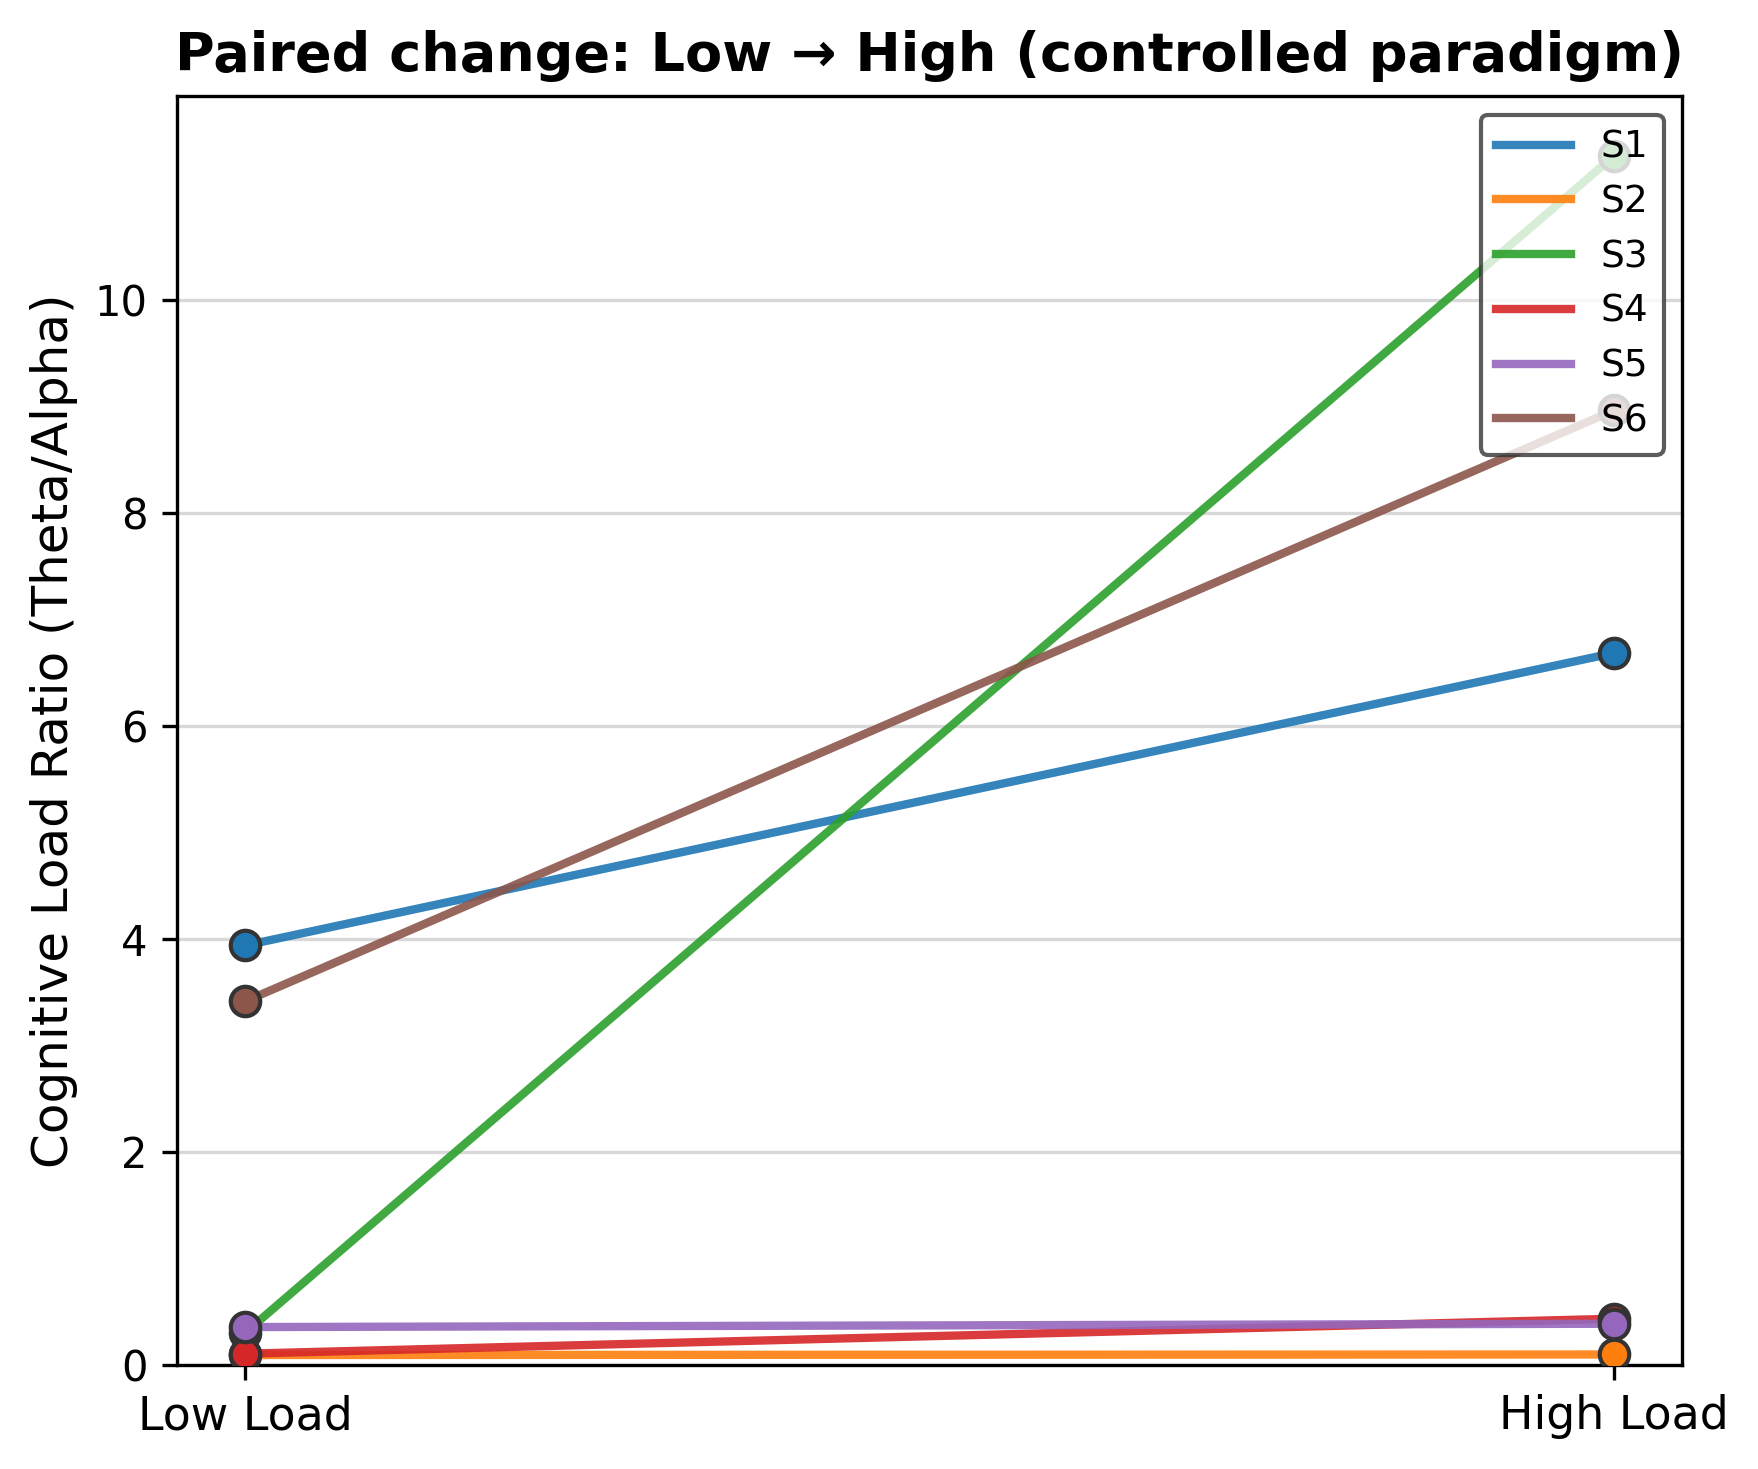
\includegraphics[width=0.7\linewidth]{figures/cumplen_incluibles_paired_slope.png}
\caption{Paired slope plot: Theta/Alpha (Fz/Pz) ratio for each of the six includable sessions from Low Load to High Load (controlled paradigm). Each line represents one session; all lines show an increase, consistent with the hypothesis.}
\label{fig:paired_slope}
\end{figure}

\subsection{Ecological paradigm: exergaming task (baseline-normalized)}

For the ecological exergaming paradigm, analysis was conducted at the session level using recordings that contained an identifiable task segment suitable for baseline comparison. The Theta/Alpha ratio was computed using the same index definition (Fz/Pz) and normalized relative to each session’s baseline value (Equation \ref{CLI}).

%\[
%\mathrm{Index}_{\mathrm{norm}} = \frac{\mathrm{Index}_{\mathrm{task}}}{\mathrm{Index}_{\mathrm{baseline}}}.
%\]
Normalized values greater than 1 indicate higher index values during the task segment relative to baseline.

Across eight analyzed sessions, six exhibited $\mathrm{Index}_{\mathrm{norm}} > 1$ (task $>$ baseline), while two sessions showed $\mathrm{Index}_{\mathrm{norm}} < 1$ (task $<$ baseline). Sessions with $\mathrm{Index}_{\mathrm{norm}} > 1$ yielded normalized ratios of 7.85, 1.87, 2.51, 3.14, 4.08, and 2.14, whereas the remaining two sessions yielded normalized ratios of 0.71 and 0.33.

Figure~\ref{fig:eco_norm} summarizes the baseline-normalized Theta/Alpha (Fz/Pz) ratio for each ecological session. Session identifiers (S1--S8) correspond to recording sessions and do not necessarily represent unique participants, as some participants completed multiple sessions using different interaction modalities. Values above unity indicate increased cognitive load during task execution relative to baseline, whereas values below unity are reported without overinterpretation and may reflect individual differences, baseline selection, or variability in task engagement.

\begin{figure}[H]
    \centering
    
\includegraphics[width=\linewidth]{figures/eco_normalized_ratio_log.png}
    \caption{Ecological paradigm: baseline-normalized Theta/Alpha (Fz/Pz) ratio during the task segment (task/baseline). The dashed line indicates the unity reference (no change relative to baseline).}
    \label{fig:eco_norm}
\end{figure}


\subsection{Subjective workload and its relationship with the EEG-based index}

NASA-TLX scores provided complementary subjective estimates of perceived workload. For the controlled paradigm, a single global NASA-TLX score was collected per participant, yielding a mean workload of 48.8\% (SD = 13.5, $N=10$). For the ecological paradigm, mean subjective workload values were 41.4\% (SD = 14.1) for Haptic, 35.3\% (SD = 13.8) for Gamepad, and 44.1\% (SD = 15.2) for Keyboard ($N=10$).

Of the six includable controlled-paradigm sessions, NASA-TLX was available for five (sessions S1, S2, S3, S5, and S6 from Table~\ref{tab:controlled}); the remaining participant did not complete the NASA-TLX questionnaire. For this subset ($N=5$), the global NASA-TLX percentage was compared with two EEG-derived quantities: the High-load Theta/Alpha mean and the within-participant difference $\Delta = \mathrm{Theta/Alpha}_{\mathrm{High}} - \mathrm{Theta/Alpha}_{\mathrm{Low}}$. NASA-TLX vs.\ the High-load index yielded a positive but non-significant correlation (Pearson $r=+0.50$, $p=0.39$; Spearman $\rho=+0.30$); NASA-TLX vs.\ $\Delta$ Theta/Alpha was likewise positive and non-significant (Pearson $r=+0.36$, $p=0.55$; Spearman $\rho=+0.30$). The direction of the association is consistent with the expectation that higher self-reported workload co-occurs with higher EEG-derived load, but the present data do not support strong inferential claims (Fig.~\ref{fig:nasatlx}).

\begin{figure}[H]
\centering
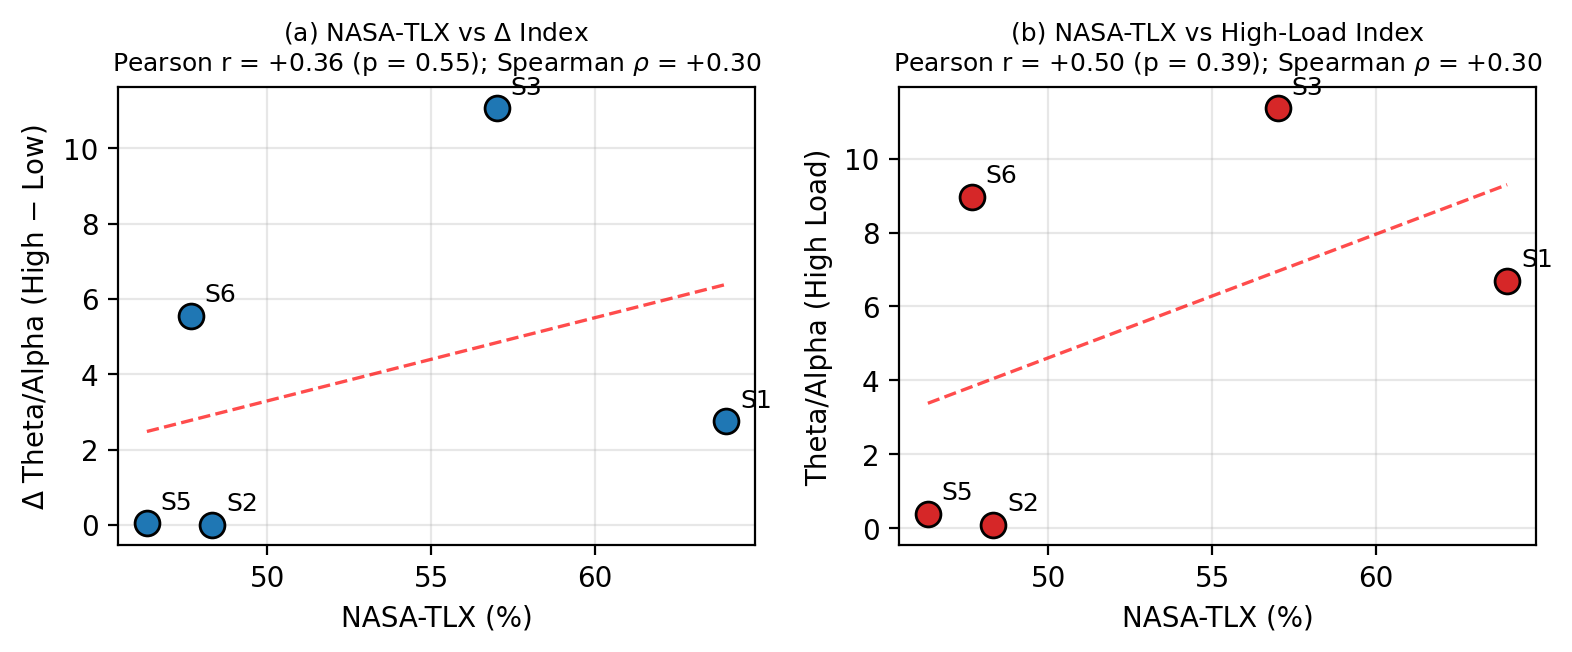
\includegraphics[width=0.9\linewidth]{figures/nasa_tlx_vs_index.png}
\caption{Exploratory relationship between subjective workload (NASA-TLX) and the EEG-based Theta/Alpha (Fz/Pz) index for the controlled-paradigm subset with both measures available (S1, S2, S3, S5, S6 from Table~\ref{tab:controlled}; $N=5$): (a) NASA-TLX vs.\ $\Delta = \mathrm{High}-\mathrm{Low}$; (b) NASA-TLX vs.\ High-load Theta/Alpha. Dashed lines: OLS fits.}
\label{fig:nasatlx}
\end{figure}


%%%%%%%%%%%%%%%%%%%%%%%%%%%%%%%%%%%%%%%%%%%%%%%%%%%%%%%%%%%%%%%%%%%%%%%%%%%%%%%%
\section{Discussion}

This study evaluated the Theta/Alpha (Fz/Pz) ratio as an index of cognitive load across a controlled laboratory benchmark and an ecological interactive task. In the controlled setting, the index consistently discriminated low (passive reading) from high (Stroop interference) cognitive load across all includable sessions, yielding a medium group-level effect size, consistent with prior work linking frontal theta increases and parietal alpha suppression to executive control, conflict monitoring, and task engagement~\cite{c1,c3,c5,c7,c9}. The present results were obtained using a predefined and explicitly reported preprocessing and artifact-handling pipeline, addressing reproducibility and stability concerns raised in recent literature~\cite{c4,c6}, which is essential when proposing user-state metrics for intelligent systems.

Beyond controlled validation, the ecological exergaming paradigm provided a structured yet interactive context for examining the same index under less constrained conditions. In the majority of analyzed sessions, baseline-normalized Theta/Alpha ratios increased during task execution, indicating sensitivity to cognitive demand associated with sustained attention and sensorimotor interaction~\cite{c2,c3}. Inter-session variability, including a subset of sessions with normalized ratios below unity, is expected in ecological paradigms and may reflect baseline selection, individual engagement strategies, learning effects, or interaction modality, underscoring the importance of normalization and session-level trend analysis rather than strict threshold-based interpretations. The exploratory comparison between NASA-TLX and the EEG-based index in the participants with both measures yielded positive but non-significant correlations (both Pearson and Spearman), indicating a consistent direction of association between subjective and objective workload but not a statistically supported convergence at this sample size; because NASA-TLX was administered as a single global score per session, it is used to contextualize perceived task demand rather than to inferentially validate the EEG index.

Several limitations should be acknowledged. The controlled paradigm was constrained by strict signal-quality criteria, resulting in a modest sample size and limited valid windows in some sessions; ecological analyses were conducted at the session level without identical exclusion thresholds, so the ecological validation remains fundamentally exploratory rather than confirmatory; short analysis windows may increase variance in spectral estimates when data availability is limited; and the NASA-TLX vs.\ Theta/Alpha comparison was performed on a small subset using a single global subjective score, restricting the evidence to a directional level. Taken together, these limitations support a conservative interpretation: under the constrained conditions examined here, the proposed index exhibits a consistent directional sensitivity to differences in cognitive workload, and further data accumulation and more rigorous validation are required before positioning it as a generalizable, implementation-ready cognitive workload indicator. Future work will focus on expanding the dataset, incorporating graded task difficulty levels, administering NASA-TLX at the phase or condition level so that direct subjective--objective correlations can be tested with adequate power, and evaluating real-time, adaptive, closed-loop human--machine interaction architectures that modulate task difficulty or feedback in response to estimated workload~\cite{c10}.


%%%%%%%%%%%%%%%%%%%%%%%%%%%%%%%%%%%%%%%%%%%%%%%%%%%%%%%%%%%%%%%%%%%%%%%%%%%%%%%%
\section{Conclusion}

This study validated the Theta/Alpha ratio computed from frontal and parietal EEG channels (Fz/Pz) as a practical and interpretable index of cognitive load across controlled and ecological contexts. Under a controlled baseline--low--high protocol, the index reliably discriminated passive reading from Stroop interference in six sessions satisfying predefined signal-quality criteria. The increase from 1.37 (SD = 1.80) to 4.65 (SD = 4.99), together with a paired Cohen’s $d = 0.75$, supports the discriminative validity of the Theta/Alpha (Fz/Pz) ratio under well-defined laboratory conditions.

Beyond controlled validation, the same index exhibited sensitivity to task engagement in an ecological interactive scenario. Baseline-normalized Theta/Alpha ratios increased in the majority of analyzed sessions, while also revealing inter-session variability characteristic of naturalistic human--machine interaction contexts. These results indicate that the proposed index can capture cognitive load dynamics beyond strictly scripted tasks when appropriate normalization and session-level analysis are applied.

Overall, and within the constrained conditions examined here, the findings support the Theta/Alpha (Fz/Pz) ratio as a compact and interpretable EEG-based metric that exhibits a consistent directional sensitivity to differences in cognitive workload, while broader generalization will require further data accumulation and more rigorous validation. This dual validation, together with an exploratory comparison against subjective NASA-TLX workload, establishes a methodological foundation for future real-time and adaptive user-state estimation frameworks in intelligent interaction environments.



%%%%%%%%%%%%%%%%%%%%%%%%%%%%%%%%%%%%%%%%%%%%%%%%%%%%%%%%%%%%%%%%%%%%%%%%%%%%%%%%
\section*{Acknowledgment}
The authors thank the Mirai Innovation Research Institute for providing the experimental infrastructure and technical support, including the AURA EEG acquisition system used in this study. The Advanced Robotics and Haptic Interfaces Laboratory (UAEH) is also acknowledged for the development and maintenance of the interactive exergaming platform employed in the ecological paradigm.

E. R. Hernandez-Rios and J. Aparicio-Juarez acknowledge the Secretariat of Science, Humanities, Technology and Innovation (SECIHTI), Mexico, for the doctoral scholarships received. O. A. Dominguez-Ramirez acknowledges support from the National System of Researchers (SNII), SECIHTI, Mexico.


%%%%%%%%%%%%%%%%%%%%%%%%%%%%%%%%%%%%%%%%%%%%%%%%%%%%%%%%%%%%%%%%%%%%%%%%%%%%%%%%
%%%%%%%%%%%%%%%%%%%%%%%%%%%%%%%%%%%%%%%%%%%%%%%%%%%%%%%%%%%%%%%%%%%%%%%%%%%%%%%%
\begin{thebibliography}{99}
\footnotesize


\bibitem{c1}
B. Raufi and L. Longo, ``An Evaluation of the EEG alpha-to-Theta and Theta-to-alpha Band Ratios as Indexes of Mental Workload,'' \emph{Front. Neuroinform.}, vol. 16, p. 861967, 2022. doi:10.3389/fninf.2022.861967

\bibitem{c2}
R. Khan, J. Vernooij, D. Salvatori, and B. P. Hierck, ``Assessing cognitive load using EEG and eye-tracking in 3-D learning environments: A systematic review,'' \emph{Multimodal Technol. Interact.}, vol. 9, no. 9, p. 99, 2025. doi:10.3390/mti9090099

\bibitem{c3}
A. D. Blanco, K. Chugani, C. Braboszcz, E. Kroupi, and A. Soria-Frisch, ``EEG spectral power correlates across cognitive tasks: Implications for VR, UXA, and Ergonomics,'' \emph{Biol. Psychol.}, vol. 200, p. 109084, 2025. doi:10.1016/j.biopsycho.2025.109084

\bibitem{c4}
S. Chikhi, N. Matton, and S. Blanchet, ``EEG power spectral measures of cognitive workload: A meta-analysis,'' \emph{Psychophysiology}, vol. 59, no. 6, p. e14009, 2022. doi:10.1111/psyp.14009

\bibitem{c5}
M. Pušica, B. Mijović, M. C. Leva, and I. Gligorijevic, ``Machine learning performance in EEG-based mental workload classification across task types: a systematic review,'' \emph{Front. Neuroergon.}, vol. 6, p. 1621309, 2025. doi:10.3389/fnrgo.2025.1621309

\bibitem{c6}
M. Mondellini, I. Pirovano, V. Colombo, S. Arlati, M. Sacco, G. Rizzo, and A. Mastropietro, ``A multimodal approach exploiting EEG to investigate the effects of VR environment on mental workload,'' \emph{Int. J. Hum.-Comput. Interact.}, vol. 40, no. 19, pp. 6566--6578, 2024. doi:10.1080/10447318.2023.2258017

\bibitem{c7}
S. Moontaha et al., ``Wearable EEG-based cognitive load classification by personalized and generalized model using brain asymmetry,'' in \emph{Proc.\ 16th Int.\ Joint Conf.\ on Biomedical Engineering Systems and Technologies---HEALTHINF}, 2023. doi:10.5220/0011628300003414

\bibitem{c8}
E. Tan, S. V. Troller-Renfree, S. Morales, G. A. Buzzell, M. McSweeney, M. Antúnez, and N. A. Fox, ``Theta activity and cognitive functioning: Integrating evidence from resting-state and task-related developmental electroencephalography (EEG) research,'' \emph{Dev. Cogn. Neurosci.}, vol. 67, p. 101404, 2024. doi:10.1016/j.dcn.2024.101404

\bibitem{c9}
J. Wu, Z. Guan, C. Li, et al., ``Brain functional connectivity after Stroop task induced cognitive fatigue,'' \emph{Sci. Rep.}, vol. 15, p. 22342, 2025. doi:10.1038/s41598-025-08330-6

\bibitem{c10}
N. I. Arana-De Las Casas, D. Sáenz-Zamarrón, A. A. Maldonado-Macías, and J. De la Riva-Rodríguez, ``Real-time mental workload measurement for four break configurations in cognitive tasks using the EEG-based workload index (EWI),'' \emph{Research Square (Preprint)}, 2024. doi:10.21203/rs.3.rs-4442355/v1

\bibitem{14}
A. Serrano-Barroso et al., ``Detecting attention levels in ADHD children with a video game,'' \emph{Sensors}, vol. 21, no. 9, p. 3221, 2021. doi:10.3390/s21093221

\bibitem{15}
H. Ji et al., ``The Effects of Exergaming on Attention in Children With ADHD,'' \emph{JMIR Serious Games}, vol. 11, p. e40438, 2023. doi:10.2196/40438

\bibitem{16}
B. Tleubayev et al., ``Robot-assisted therapy for children with ADHD and ASD,'' \emph{ACM ICPS}, pp. 58–62, 2019. doi:10.1145/3325693.3325703

\bibitem{22} 
O. A. Dominguez-Ramirez and V. Parra-Vega, ``Active haptic exploration of deformable objects,'' \emph{DAAAM Int. Scientific Book}, pp. 177–190, 2006.

\bibitem{23} 
O. A. Dominguez-Ramirez and V. Parra-Vega, ``Texture, Roughness and Shape Haptic Perception,'' \emph{Proc. IEEE/RSJ IROS}, 2003. doi:10.1109/IROS.2003.1249634

\bibitem{24}
A. Almukhtar, V. Caddick, R. Naik, M. Goble, G. Mylonas, A. Darzi, 
F. Orihuela-Espina, and D. R. Leff, 
``Objective Assessment of Cognitive Workload in Surgery: A Systematic Review,'' 
\emph{Ann. Surg.}, vol. 281, no. 6, pp. 942--951, Jun. 2025, 
doi: 10.1097/SLA.0000000000006370.


\end{thebibliography}

\end{document}
